\documentclass%
%[handout]
{beamer}
% % % % % % % %
% % % % % % % %
% % % % % % % %
%IMPORTANT
%compiles with
%pdflatex -shell-escape
%IMPORTANT
% % % % % % % %
% % % % % % % %
% % % % % % % %
\mode<presentation>
{
\useinnertheme{rounded}
\useoutertheme{infolines}
\usecolortheme{orchid}
\usecolortheme{whale}
}

\usepackage[english]{babel}
\usepackage[latin1]{inputenc}
\usepackage[all,cmtip]{xy}
\usepackage{times}
\usepackage[T1]{fontenc}
\usepackage{../example-templates}
\usepackage{../pstricks-commands}

\usepackage{auto-pst-pdf}
\usepackage{pst-plot}
%\usepackage{pstricks-add}

% Or whatever. Note that the encoding and the font should match. If T1
% does not look nice, try deleting the line with the fontenc.


\graphicspath{{../../modules/}}

\newtheoremstyle{partialproof}{3pt}{3pt}{}{}{}{.}{.5em}{}
\theoremstyle{partialproof} \newtheorem{partialproof}[theorem]{Proof.}
%\DeclareMathOperator{\diff}{d}
\setbeamertemplate{navigation symbols}{}

\includeonlylecture{1}

\newcommand{\lect}[3]{
  \date{#1}
  \lecture[#1]{#2}{#3}
}

\setbeamertemplate{footline}
{
  \leavevmode%
  \hbox{%
  \begin{beamercolorbox}[wd=.333333\paperwidth,ht=2.25ex,dp=1ex,center]{author in head/foot}%
    \usebeamerfont{author in head/foot}\insertshortauthor
  \end{beamercolorbox}%
  \begin{beamercolorbox}[wd=.333333\paperwidth,ht=2.25ex,dp=1ex,center]{title in head/foot}%
    \usebeamerfont{title in head/foot}\insertshorttitle
  \end{beamercolorbox}%
  \begin{beamercolorbox}[wd=.333333\paperwidth,ht=2.25ex,dp=1ex,center]{date in head/foot}%
    \usebeamerfont{date in head/foot}\insertshortdate{}
  \end{beamercolorbox}}%
  \vskip0pt%
}

% If you have a file called "university-logo-filename.xxx", where xxx
% is a graphic format that can be processed by latex or pdflatex,
% resp., then you can add a logo as follows:

%\pgfdeclareimage[height=0.8cm]{logo}{bluelogo}
%\logo{\pgfuseimage{logo}}
\renewcommand{\Arcsin}{\arcsin}
\renewcommand{\Arccos}{\arccos}
\renewcommand{\Arctan}{\arctan}
\renewcommand{\Arccot}{\text{arccot\hspace{0.03cm}}}
\renewcommand{\Arcsec}{\text{arcsec\hspace{0.03cm}}}
\renewcommand{\Arccsc}{\text{arccsc\hspace{0.03cm}}}



\begin{document}

\AtBeginLecture{%

\title[\insertlecture]{FreeCalc}
\subtitle{\insertlecture}
\author[FreeCalc]{}
\institute[UMass Boston]{University of Massachusetts Boston}
\date{\insertshortlecture}
\begin{frame}
  \titlepage
\end{frame}
}%

% begin lecture
\lect{\today}{Sample}{1}{
\begin{frame}
 \frametitle{Spherical Coordinates}
\begin{columns}
\column{0.55\textwidth}
%  \psfrag{P}{$P$}
%  \psfrag{O}{$O$}  
%  \psfrag{xp}{$x_P$} 
%  \psfrag{yp}{$y_P$} 
%  \psfrag{zp}{$z_P$}     
%  \psfrag{rho}{$\rho_P$}
%  \psfrag{thp}{$\theta_P$}
%  \psfrag{phi}{$\phi_P$}
\psset{xunit=1cm, yunit=1cm}
\begin{pspicture}(-2,-2.5)(2,2)
\tiny
\renewcommand{\fcScreen}{[-1 -0.4 -0.25] -1}
\fcBoundingBox{-2}{-2.5}{2}{2}
\fcAxesIIId{5}{5}{5}
\fcPutIIId[r]{[0 -0.15 0.15]}{$O$}
\fcLineIIId[linestyle=dotted]{[3 0 0]}{[3 3 0]}
\fcLineIIId[linestyle=dotted]{[3 3 0]}{[0 3 0]}
\fcLineIIId[linestyle=dotted]{[0 0 0]}{[0 3 0]}
\fcLineIIId{[0 0 0]}{[3 3 0]}
\fcLineIIId{[3 3 0]}{[3 3 3]}
\fcLineIIId{[0 0 3]}{[3 3 3]}
\fcPutIIId[l]{[3.1 3.1 3.1]}{$P$}
\fcPutIIId[r]{[1.5 -0.1 0]}{$x_P$}
\fcPutIIId[t]{[3 3 0]}{$Q$}
\fcPutIIId[b]{[0 1.5 0]}{$y_P$}
\fcPutIIId[l]{[3 3 1.5]}{$~~z_P$}
\fcPutIIId[r]{[0 0 1.5]}{$z_P~~$}
\uncover<2->{%
\fcLineIIId{[0 0 0]}{[3 3 3]}
\uncover<3>{\fcLineIIId[linecolor=red, linewidth=2pt]{[0 0 0]}{[3 3 3]}}%
\fcPutIIId[r]{[2.1 2.1 2.1]}{$\rho_P$}
\fcPutIIId[rt]{[1 1 1.5]}{$\phi_P~~$}
\fcPutIIId[tr]{[1.8 0.9 0]}{$\theta_P$}%
\fcAngleIIId[linecolor=red, arrows=->]{[0 0 1]}{[3 3 3]}{1.7}%
\uncover<4>{\fcAngleIIId[linecolor=red, linewidth=2pt, arrows=->]{[0 0 1]}{[3 3 3]}{1.7}}%
\fcAngleIIId[linecolor=red, arrows=->]{[1 0 0]}{[3 3 0]}{1.7}%
\uncover<5>{\fcAngleIIId[linecolor=red, arrows=->, linewidth=2pt]{[1 0 0]}{[3 3 0]}{1.7}}%
}%
\uncover<8>{\fcLineIIId[arrows=->, linecolor=red, linewidth=2pt]{[0 0 0]}{[5 5 5]}}%
\uncover<10>{%
\fcAngleIIId[linecolor=red, linewidth=2pt]{[0 0 1]}{[1 1 0]}{2}%
\fcAngleIIId[linecolor=red, linewidth=2pt, arrows=->]{[1 1 0]}{[0 0 -1]}{2}%
}%
\uncover<12>{%
\fcAngleIIId[linecolor=red, linewidth=2pt]{[1 0 0]}{[0 1 0]}{2}%
\fcAngleIIId[linecolor=red, linewidth=2pt]{[0 1 0]}{[-1 0 0]}{2}%
\fcAngleIIId[linecolor=red, linewidth=2pt]{[-1 0 0]}{[0 -1 0]}{2}%
\fcAngleIIId[linecolor=red, linewidth=2pt, arrows=->]{[0 -1 0]}{[1 0 0]}{2}%
}%
\end{pspicture}   
%  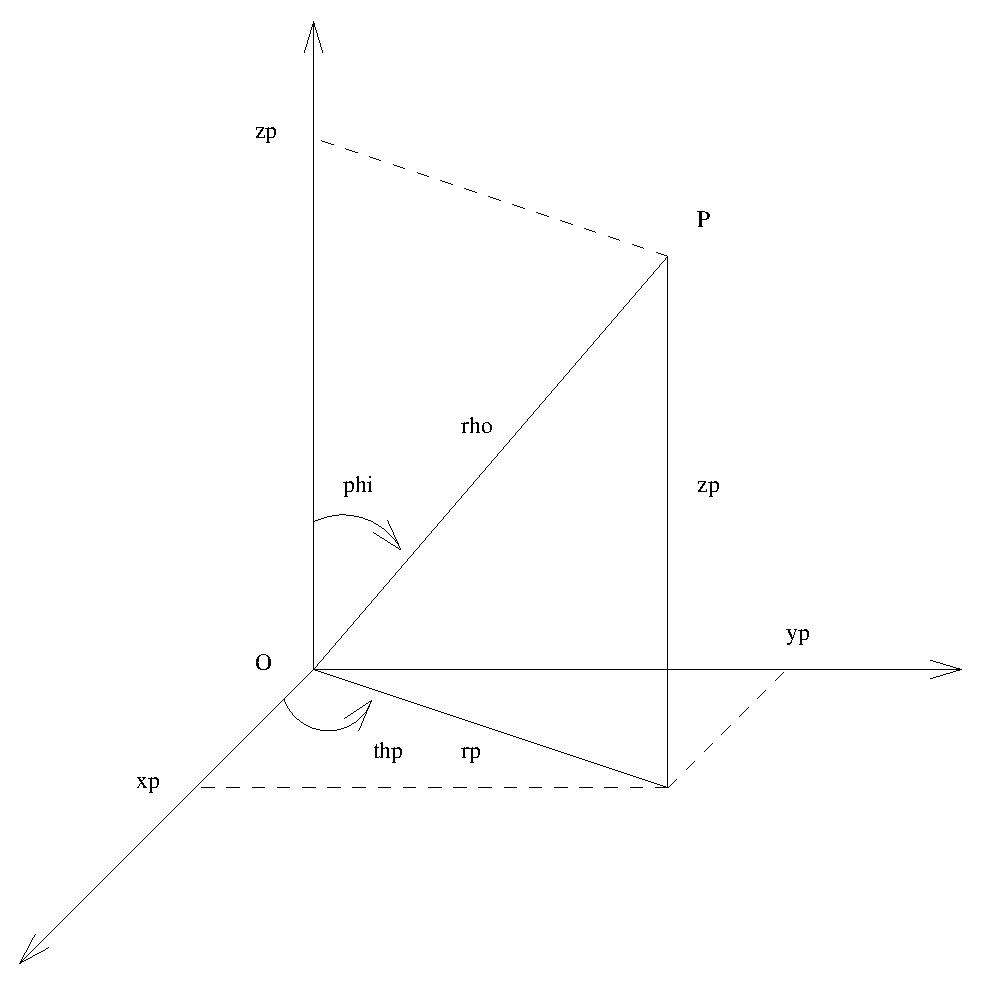
\includegraphics[height=2in]{../../modules/coordinate-systems/pictures/ok-cylindrical-spherical.eps}
\column{0.45\textwidth}
	\begin{itemize}
\item In Cartesian coordinates, a point $P$ is given by triple $(x_P, y_P, z_P)$.
\item<2-> We introduce alternative spherical coordinates $(\rho_P, \phi_P,\theta_P)$.
\begin{itemize}
\item \alert<3>{$\rho_P$: distance $|OP|$;}
\item \alert<4>{$\phi_P$: angle $Oz$ to $OP$;}
\item \alert<5>{$\theta_P$: angle $Ox$ to $OP_{xy}$.}
\end{itemize}
\item<6-> Coordinates range:
\begin{itemize}
\item \alert<7,8>{$\rho$:} \uncover<8->{\alert<8>{ $[0,\infty)$;}}
\item \alert<9,10>{$\phi$:}  \uncover<10->{\alert<10>{$[0, \pi]$;}}
\item \alert<11,12>{$\theta$:}  \uncover<12->{ \alert<12>{$[0,2\pi)$.}}
\end{itemize}
\end{itemize}
\end{columns}
\end{frame}

%\begin{frame}
\begin{pspicture}(-1, -1)(2,2)
\fcBoundingBox{-1}{-1}{2}{2}
\fcSurfaceDirectDraw{iterationsX=10, iterationsY=10, Delta=1}{-90}{-1}{90}{1}{[u cos u sin v]}
\end{pspicture}
\begin{pspicture}(-1, -1)(2,2)
\fcBoundingBox{-1}{-1}{2}{2}
\fcStartIIIdScene %
\fcSurfaceInScene[iterationsU=7, iterationsV=4]{0}{-1}{300}{1}{[u cos u sin v]}
\fcFinishIIIdScene
\end{pspicture}
\end{frame}

%\begin{frame}
\begin{pspicture}(-2,-2)(2,2)
%\pstVerb{[1 5 6]  \fcArrayToStack stack}
\pstVerb{[1 2 3] \fcProjectOntoScreen ==}
\pstVerb{[1 2 3] [4 5 6] \fcVectorMinusVector ==}
%\fcFullDot{1}{1}
%\pstVerb{[1 2 3] 5 \fcVectorTimesScalar \fcArrayToStack stack}
%\pscircle*[fillcolor=white, linecolor=red](! \fcProjectOriginOnPlane{1}{1}{1}{1}){0.07}
\end{pspicture}
\end{frame}
%\begin{frame}
Looking for $t $ such that 
\[
\begin{array}{rcl}
\displaystyle\langle \mathbf{v}+t \mathbf{n}, \mathbf{n}\rangle  &=&\displaystyle d\\
\displaystyle t&=&\displaystyle \frac{d-\langle\mathbf{v},\mathbf{n} \rangle}{\langle\mathbf{n}, \mathbf{n} \rangle}
\end{array}
\]
\begin{pspicture}(-2,-2)(2,2)
%\pstVerb{[1 5 6]  \fcArrayToStack stack}

\pstVerb{[1 2 3] [4 5 6] 7 \fcProjectOntoPlane \fcArrayToStack stack}

%\pstVerb{[1 2 3] 5 \fcVectorTimesScalar \fcArrayToStack stack}
%\pscircle*[fillcolor=white, linecolor=red](! \fcProjectOriginOnPlane{1}{1}{1}{1}){0.07}


\end{pspicture}
\end{frame}
%\begin{frame}
\begin{pspicture}(-2,-2)(2,2)
\fcAxesIIId{2}{2}{2}
\end{pspicture}
\end{frame}
%\begin{frame}
\psset{xunit=1cm, yunit=1cm}
\begin{pspicture}(0,0)(1,1)
\psline(0,0.1)(1, 0.1)
\psline(0,-0.1)(1,-0.1)
\fcLine{[0 0] [1 1]}
\end{pspicture}
%\begin{pspicture}(-1,-1)(1,1)
%\end{pspicture}

\end{frame}
%\begin{frame}
We have the ellipsoid 
\[
\frac{x^2}{a^2}+\frac{y^2}{b^2}+\frac{z^2}{c^2}= 1.
\]
We are seeking to project it orthographically onto the plane 
\[
px+qy+rz=s.
\]
The direction in which our ``orthographic eye'' is looking is $\fcv n= (p,q,r)$.
\end{frame}
\begin{frame}
\begin{pspicture}(0,0)(0,0)%
%\renewcommand{\fcScreenStyle}{x}%
%\renewcommand{\fcScreen}{[-1 1 2] 0}
\fcAxesIIId{5}{5}{5}%
\fcStartIIIdScene%
%\fcCurveIIIdBlockedByScreen{0}{360}{[t cos t sin 0]}{\fcScreenWithSpace pop 0}
\fcEllipsoid[linecolor=red]{0 0 0 3 2 1}%
%\fcCone{-2 2 0 0 0 1 1 1}
\renewcommand{\fcIterationsX}{15}
\renewcommand{\fcIterationsY}{15}
\fcFinishIIIdScene%
\end{pspicture}
\end{frame}
%\begin{frame}

\psset{xunit=0.4cm, yunit=0.4cm}
\begin{pspicture}(-5,-5)(5,5)
\fcAxesStandard{-5}{-5}{5}{5}
\fcVectorField[linecolor=blue, arrows=->]{startX=-5, startY=-5, Delta=1, iterationsX=11, iterationsY=11}{1 dict begin /r x x mul y y mul add sqrt def  r 0 eq {0 0} {-1 y mul r div  x r div} ifelse end}
\end{pspicture}

\end{frame}

}
\end{document}
